% Copyright 2004 by Till Tantau <tantau@users.sourceforge.net>.
%
% In principle, this file can be redistributed and/or modified under
% the terms of the GNU Public License, version 2.
%
% However, this file is supposed to be a template to be modified
% for your own needs. For this reason, if you use this file as a
% template and not specifically distribute it as part of a another
% package/program, I grant the extra permission to freely copy and
% modify this file as you see fit and even to delete this copyright
% notice. 

\documentclass{beamer}


\usepackage[utf8]{inputenc}
\usepackage[spanish]{babel}
\usepackage{lmodern}

\usepackage{graphicx}
\usepackage{multicol}
\usepackage{mathtools}
\usepackage{hyperref}
\usepackage{listings}
\usepackage{verbatim}
\usepackage{afterpage}
\usepackage{lscape}

\usepackage{amsmath}

\usepackage{cite}



% Establecemos el tema a utilizar. 
% Debe existir el archivo udpthesisEIT.sty en su sistema TeX para poder utilizarlo.

%%%%%%%%%%%%%%%%%%%%%%%%%%%%%%%
\usepackage{xspace}
\makeatletter
\DeclareRobustCommand\onedot{\futurelet\@let@token\@onedot}
\def\@onedot{\ifx\@let@token.\else.\null\fi\xspace}

\def\eg{\emph{e.g}\onedot} \def\Eg{\emph{E.g}\onedot}
\def\ie{\emph{i.e}\onedot} \def\Ie{\emph{I.e}\onedot}
\def\cf{\emph{c.f}\onedot} \def\Cf{\emph{C.f}\onedot}
\def\etc{\emph{etc}\onedot} \def\vs{\emph{vs}\onedot}
\def\wrt{w.r.t\onedot} \def\dof{d.o.f\onedot}
\def\etal{\emph{et al}\onedot}
\def\adhoc{\emph{ad hoc}\xspace}
\makeatother

\usepackage{amsthm}
% declare my operator
\usepackage{scalerel}
\DeclareMathOperator*{\cat}{\scalerel*{\|}{\sum}}



% There are many different themes available for Beamer. A comprehensive
% list with examples is given here:
% http://deic.uab.es/~iblanes/beamer_gallery/index_by_theme.html
% You can uncomment the themes below if you would like to use a different
% one:
%\usetheme{AnnArbor}
%\usetheme{Antibes}
%\usetheme{Bergen}
%\usetheme{Berkeley}
%\usetheme{Berlin}
%\usetheme{Boadilla}
%\usetheme{boxes}
%\usetheme{CambridgeUS}
%\usetheme{Copenhagen}
%\usetheme{Darmstadt}
%\usetheme{default}
%\usetheme{Frankfurt}
%\usetheme{Goettingen}
%\usetheme{Hannover}
%\usetheme{Ilmenau}
%\usetheme{JuanLesPins}
%\usetheme{Luebeck}
\usetheme{Madrid}
%\usetheme{Malmoe}
%\usetheme{Marburg}
%\usetheme{Montpellier}
%\usetheme{PaloAlto}
%\usetheme{Pittsburgh}
%\usetheme{Rochester}
%\usetheme{Singapore}
%\usetheme{Szeged}
%\usetheme{Warsaw}

\title{Reconocimiento de expresiones faciales en imágenes dinámicas utilizando un descriptor basado en rayos de flujo}

% A subtitle is optional and this may be deleted
%\subtitle{Optional Subtitle}

\author{Miguel Antonio Rodríguez Santander}
% - Give the names in the same order as the appear in the paper.
% - Use the \inst{?} command only if the authors have different
%   affiliation.

\institute[Universidad Diego Portales] % (optional, but mostly needed)
{%
  Universidad Diego Portales\\
  Facultad de Ingeniería\\
  Escuela de Informática y Telecomunicaciones
  
  % - Use the \inst command only if there are several affiliations.
% - Keep it simple, no one is interested in your street address.
}
\date{Título I\\ 30 de Julio de 2013}
% - Either use conference name or its abbreviation.
% - Not really informative to the audience, more for people (including
%   yourself) who are reading the slides online

\subject{Thesis}
% This is only inserted into the PDF information catalog. Can be left
% out. 

% If you have a file called "university-logo-filename.xxx", where xxx
% is a graphic format that can be processed by latex or pdflatex,
% resp., then you can add a logo as follows:

% \pgfdeclareimage[height=0.5cm]{university-logo}{university-logo-filename}
% \logo{\pgfuseimage{university-logo}}

% Delete this, if you do not want the table of contents to pop up at
% the beginning of each subsection:

\AtBeginSection[]
{
  \begin{frame}<beamer>{Índice}
    \tableofcontents[currentsection,currentsubsection]
  \end{frame}
}

\AtBeginSubsection[]
{
  \begin{frame}<beamer>{Índice}
    \tableofcontents[currentsection,currentsubsection]
  \end{frame}
}

% Let's get started
\begin{document}

\begin{frame}
  \titlepage
\end{frame}

\begin{frame}{Índice}
  \tableofcontents
  % You might wish to add the option [pausesections]
\end{frame}

% Section and subsections will appear in the presentation overview
% and table of contents.


% You can reveal the parts of a slide one at a time
% with the \pause command:

\section{Motivación}

\begin{frame}
  \frametitle{Motivación}
  \begin{columns}[onlytextwidth]
    \begin{column}{0.5\textwidth}
      \centering
      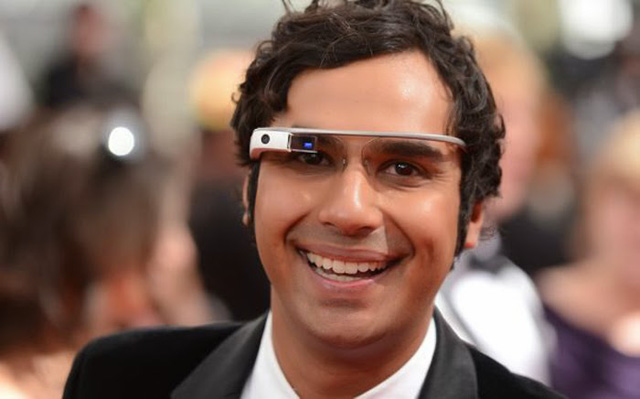
\includegraphics[width=5cm]{imagenes/google_glass.jpg}
    \end{column}
    \begin{column}{0.5\textwidth}
        \begin{itemize}
            \item Aplicaciones a distintas áreas del conocimiento humano
            \item Utilidad en tecnologías actuales
            \item 55\% en la transmisión del mensaje
        \end{itemize}
    \end{column}
  \end{columns}
\end{frame}


\section{Problema}
    
    \begin{frame}{Problema}{Expresiones faciales universales}
		  \begin{columns}[onlytextwidth]
    		  	\begin{column}{0.7\textwidth}
      			\centering
      			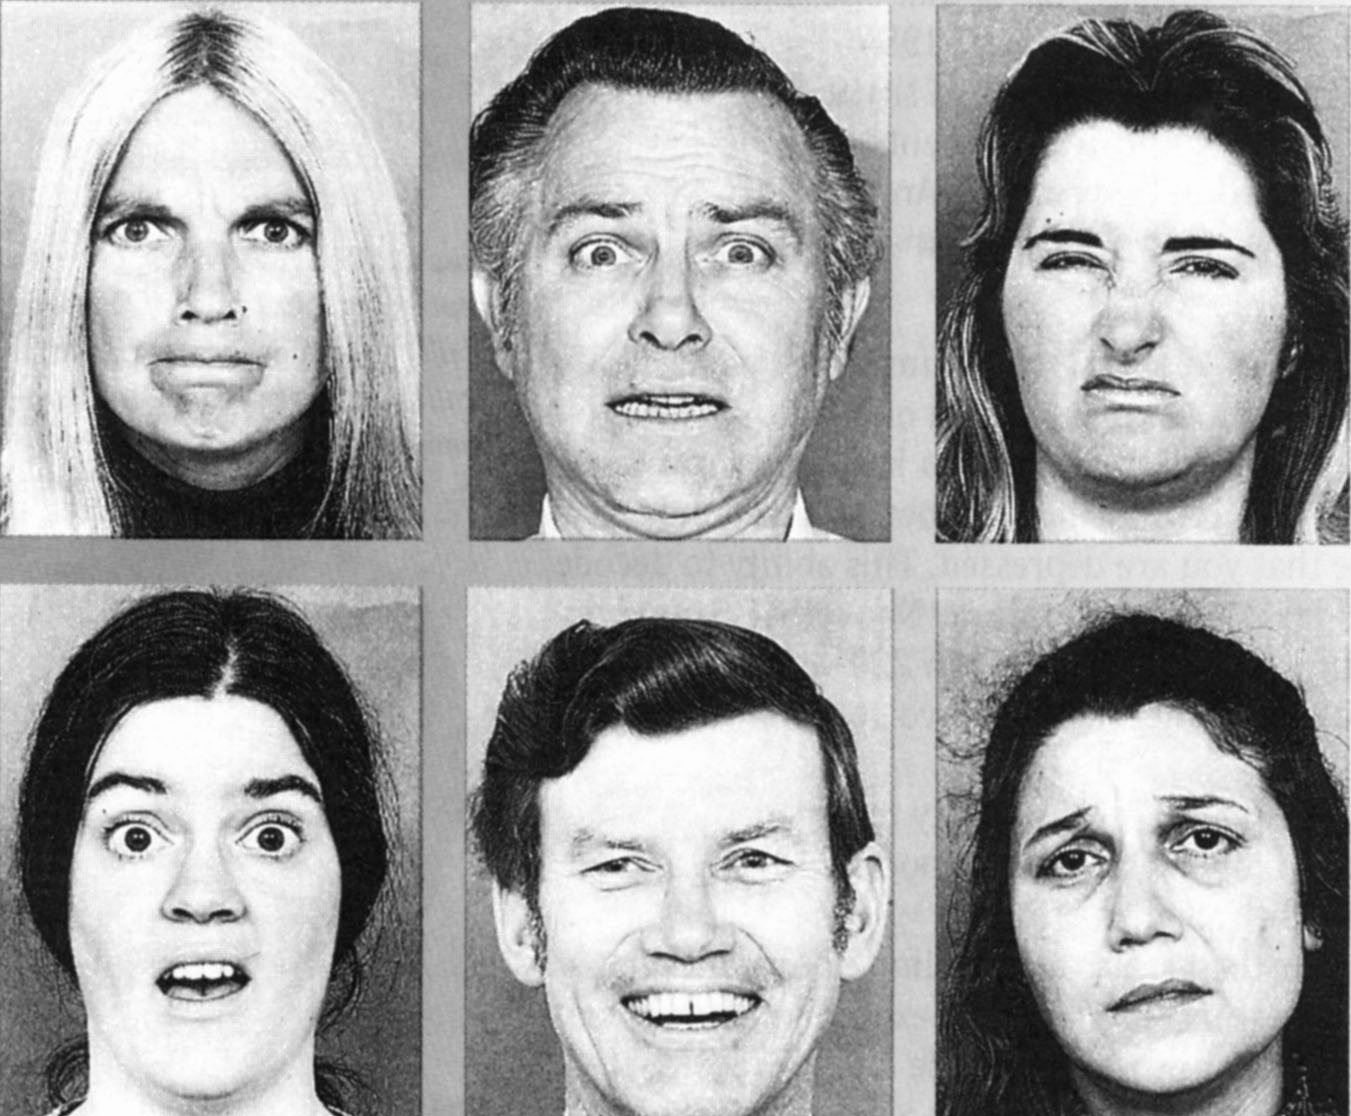
\includegraphics[width=7cm]{imagenes/expresiones_faciales_universales.jpg}
    			\end{column}
    		    \begin{column}{0.3\textwidth}
        	      \begin{itemize}
            	    \item Alegría
            		\item Asco
            		\item Ira
            		\item Miedo
            		\item Sorpresa
            		\item Tristeza
        	   	  \end{itemize}
            \end{column}
          \end{columns}          
          
          
          
    \end{frame}
    

    \subsection{Soluciones}
        \begin{frame}{Métodos Geométricos}
              \centering
                Hablar algo de esto
        \end{frame}
    
        \begin{frame}{Métodos de apariencia}{Local Binary Patterns}
            \begin{figure}[bt]
        		\centering
                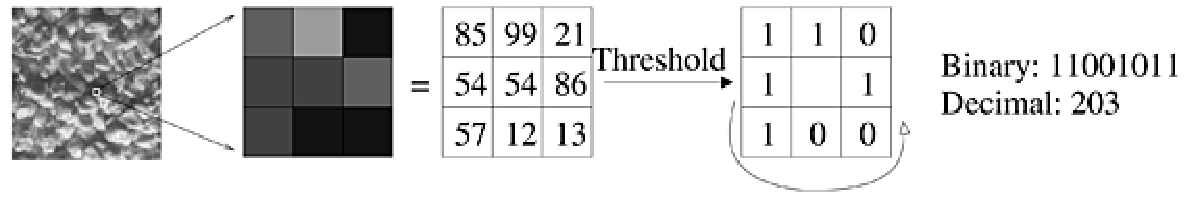
\includegraphics[width=9cm]{imagenes/lbp.pdf}
          		\caption{Codificación LBP.}
            \end{figure}	

            \begin{figure}[bt]
        		\centering
                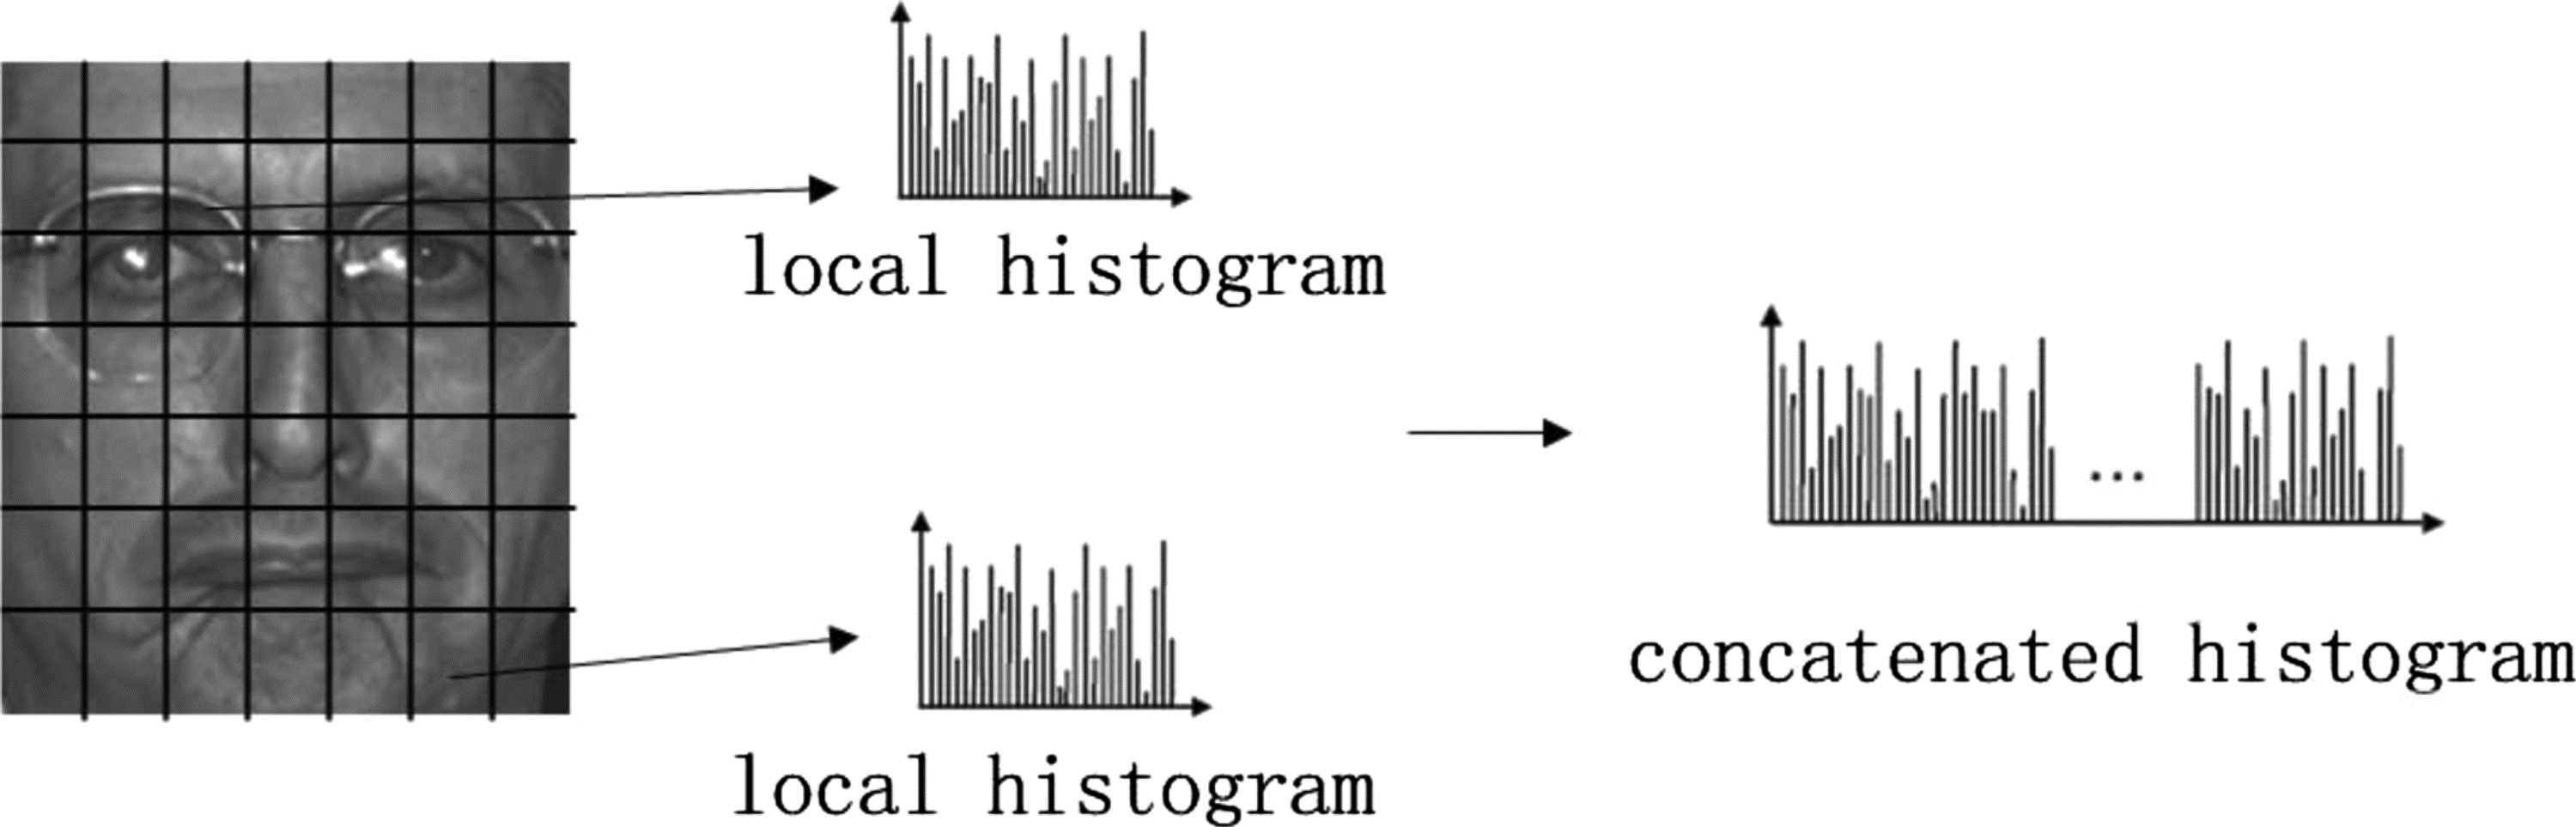
\includegraphics[width=9cm]{imagenes/lbp_histogram.png}
          		\caption{Creación del descriptor utilizando LBP.}
            \end{figure}	  
        \end{frame}
        
        \begin{frame}{Métodos de apariencia}{Local Direccional Number Patterns}
            \begin{figure}[bt]
        		\centering
                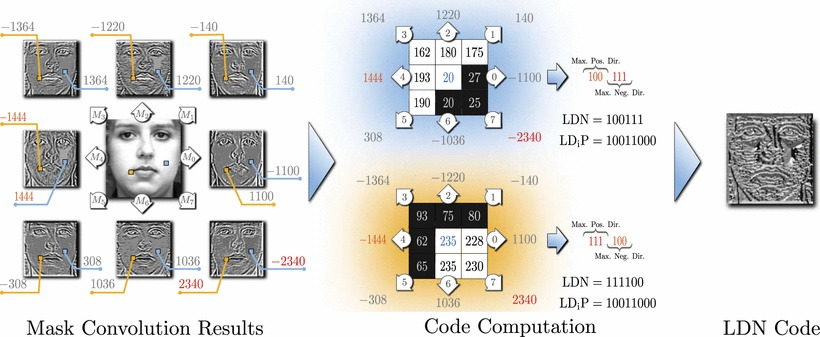
\includegraphics[width=9cm]{imagenes/ldn.jpg}
          		\caption{Codificación LDN.}
            \end{figure}
        \end{frame}
        
        
        \begin{frame}{Métodos de apariencia}{Volume Local Binary Patterns}
            \begin{figure}[bt]
        		\centering
                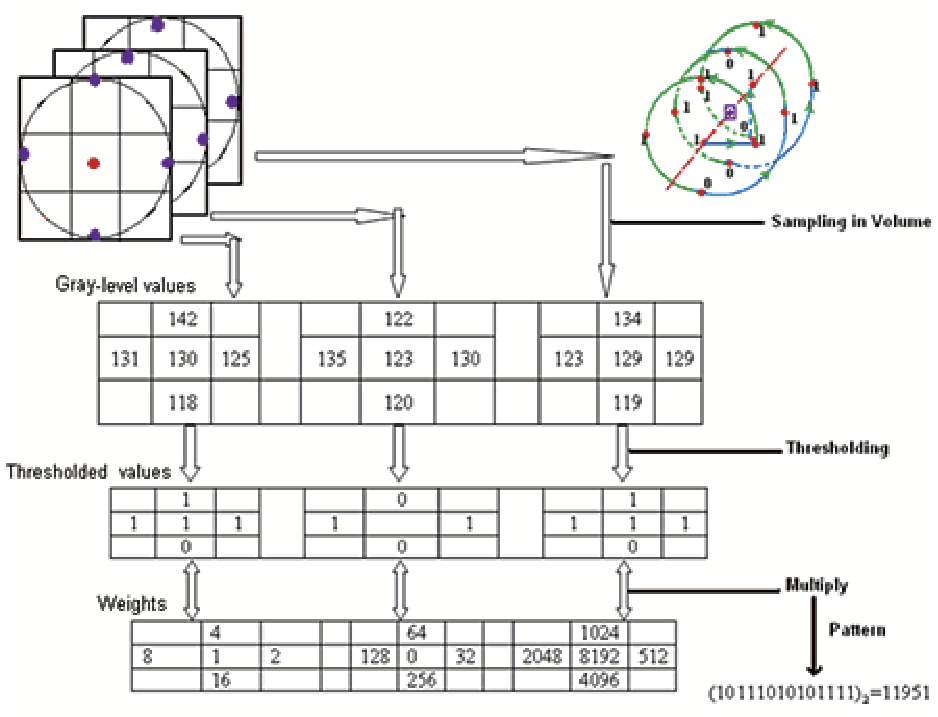
\includegraphics[width=8cm]{imagenes/vlbp.pdf}
          		\caption{Codificación VLBP.}
            \end{figure}
        \end{frame}
    
        
        \begin{frame}{Métodos de apariencia}{Local Binary Patterns- Three Ortogonal Planes}
            \begin{figure}[bt]
        		\centering
                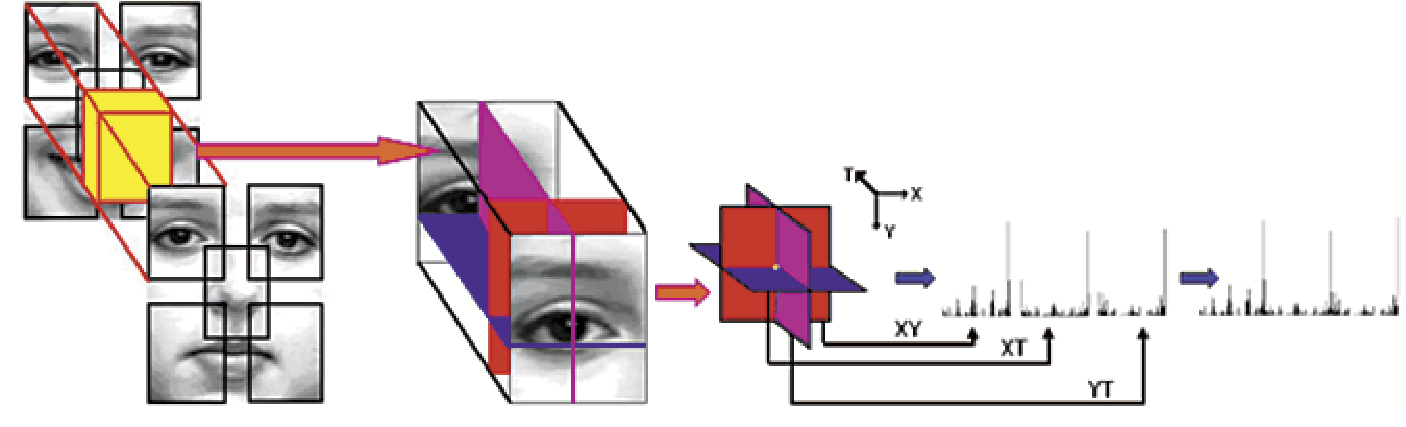
\includegraphics[width=9cm]{imagenes/lbptop.pdf}
          		\caption{Codificación LBP-TOP.}
            \end{figure}
        \end{frame}
    

\section{Solución propuesta}
	\subsection{Pipeline}    
    \begin{frame}{Solución propuesta}{Pipeline}
        \begin{figure}[bt]
    		\centering
            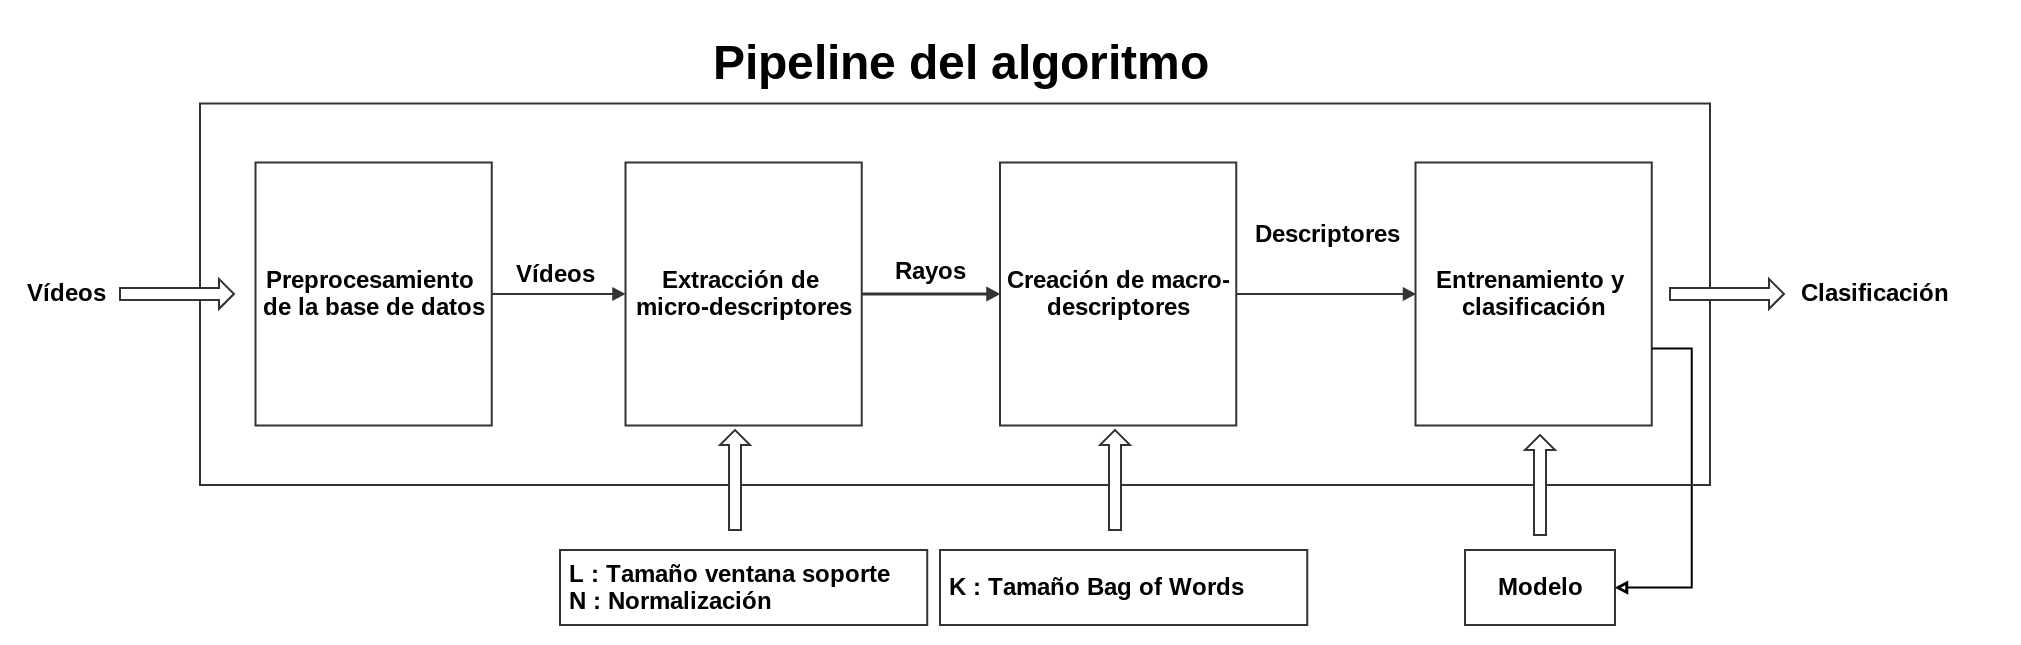
\includegraphics[width=12cm]{imagenes/pipeline.png}
      		\caption{Método propuesto.}
        \end{figure}
    \end{frame}

	\subsection{Ventajas potenciales del método}
		\begin{frame}{Solución propuesta}{Ventajas potenciales del método}
			\begin{itemize}
				\item ¿Permitirán los \textit{rayos} solucionar el problema de la variable temporal?
				\item Al ser un modelado espacio-temporal de los píxeles, los \textit{rayos}, ¿permitirán ver cual es el comportamiento de los píxeles a través del tiempo?
				\item ¿Permitirán los \textit{rayos} modelar micro-patrones en los movimientos del rostro que no pueden ser vistos a simple vista por los humanos?, de ser cierto, ¿estos micro-patrones aportaran mayor información al modelo de clasificación?.
				\item ¿Existe la posibilidad de que cada una de las expresiones faciales universales pueda tener asociado un conjunto de \textit{rayos} tipo?. 
			\end{itemize}
		\end{frame}	
	
	
    \subsection{Preprocesamiento de la base de datos}
        \begin{frame}{Preprocesamiento de la base de datos}
        
            \begin{columns}[onlytextwidth]
                \begin{column}{0.4\textwidth}
                    \begin{itemize}
                        \item Detección de rostros
                        \item Corrección de movimiento
                    \end{itemize}
                \end{column}
                \begin{column}{0.6\textwidth}
                    \begin{figure}[bt]
                		\centering
                        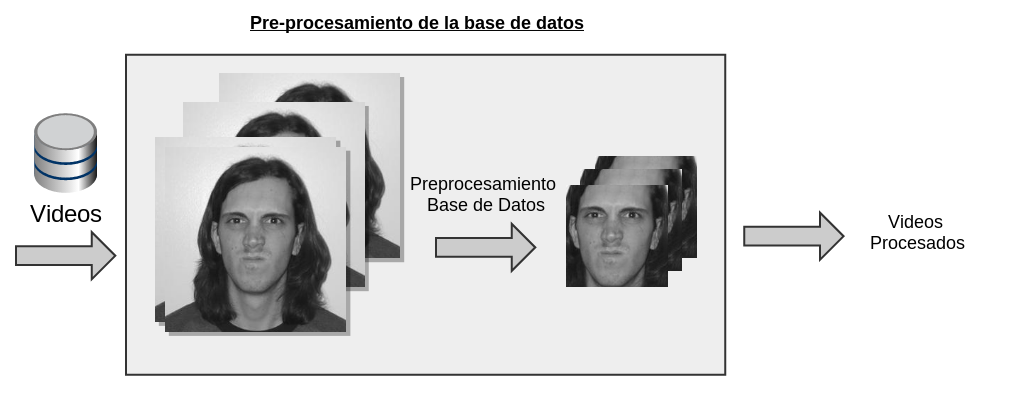
\includegraphics[width=7cm]{imagenes/Preprocesamiento.png}
                  		\caption{Preprocesamiento de la base de datos.}
                    \end{figure}
                \end{column}
            \end{columns}
        
        \end{frame}
    
    
    
    \subsection{Extracción de micro-descriptores}
        \begin{frame}{Extracción de micro-descriptores}{Vista general}
            \begin{figure}[bt]
        		\centering
                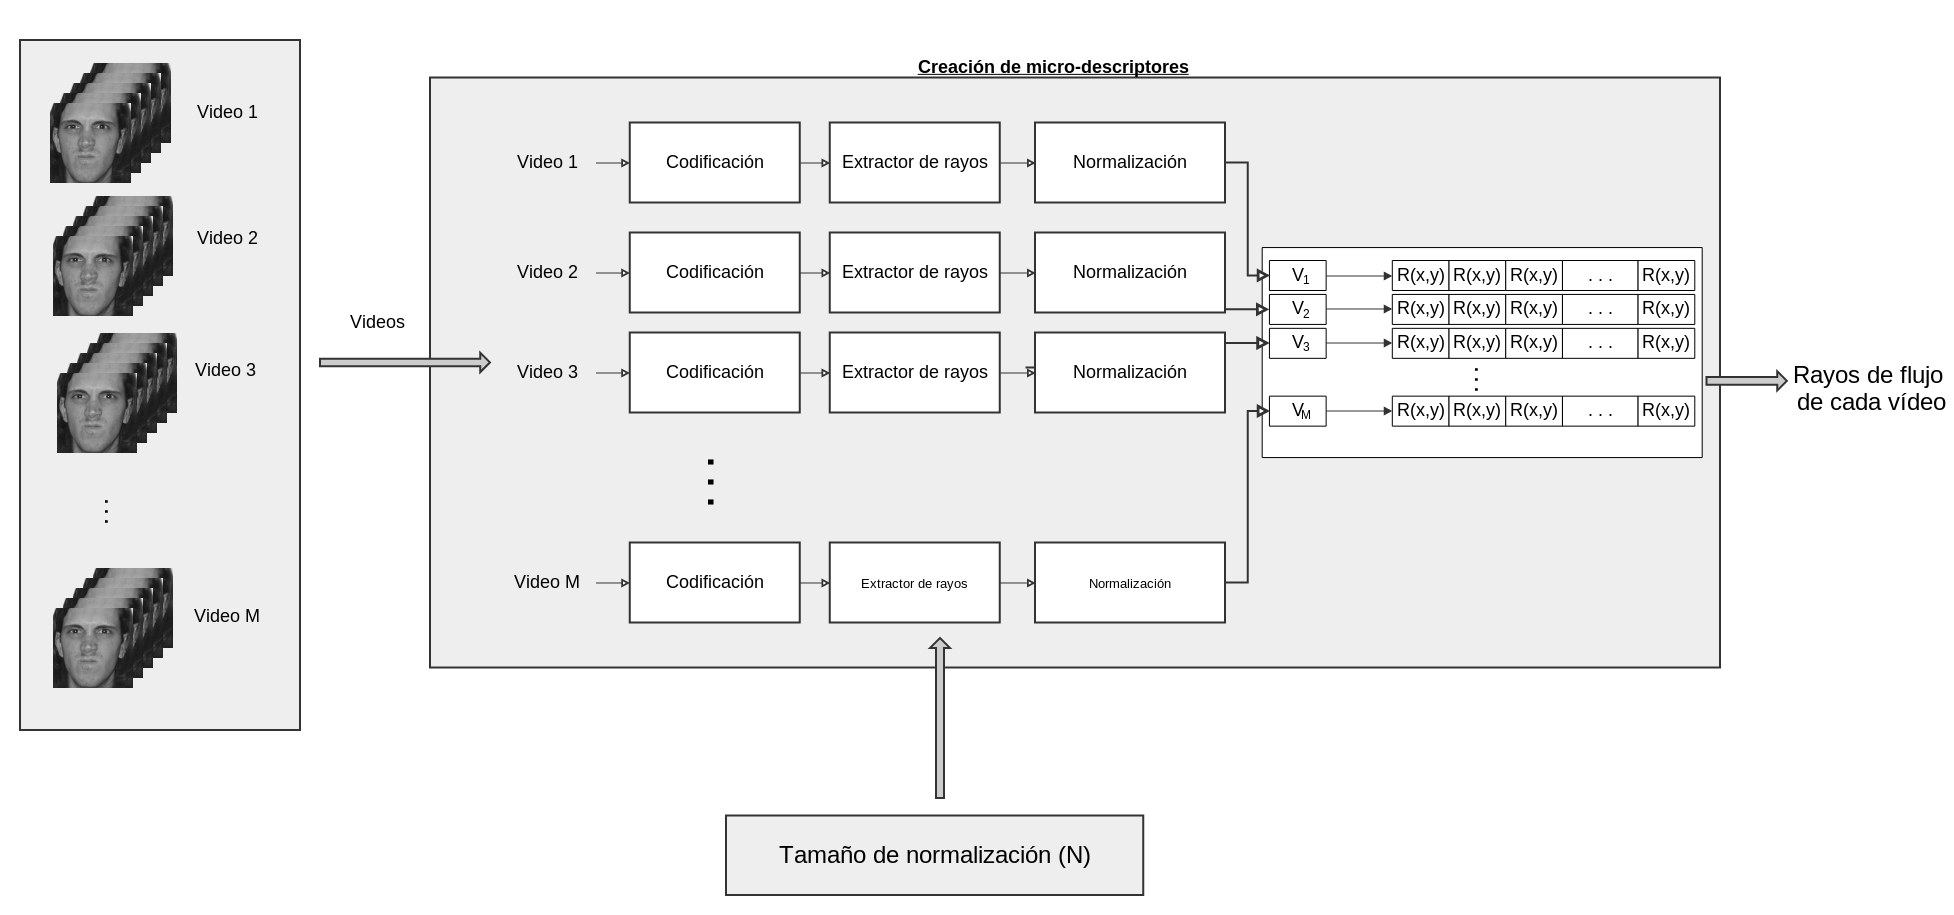
\includegraphics[width=12cm]{imagenes/Extractor_microdescriptores.png}
          		\caption{Diagrama general del proceso de extracción de micro-descriptores.}
            \end{figure}
        \end{frame}
    
    
        \begin{frame}{Extracción de micro-descriptores}{Extracción de rayos}
            \begin{block}{Región de soporte}
                  Dado un píxel $(x,y)$ en un cuadro $t$, definimos una región de soporte RS, de tamaño $L \times L$ (donde $L$ es impar), como la subregión del cuadro $t$ que está centrada en el píxel $(x,y)$.
            \end{block}
            
            \begin{block}{Ventana de búsqueda}
                  Dado un píxel $(x,y)$ en un cuadro $t$, definimos la ventana de búsqueda WS, de  tamaño $(2L+1) \times (2L+1)$, como la subregión del cuadro $t+1$ que está centrada en el píxel $(x,y)$.
            \end{block}
    
        \end{frame}
    

        \begin{frame}{Extracción de micro-descriptores}{Extracción de rayos}
            \begin{equation}\label{algoritmo:eq:mse}	
			    \text{MSE}(\text{RS}, \text{RS}') = \sum_{x=1}^{L} \sum_{y=1}^{L} (\text{RS}(x,y,t) - \text{RS}'(x',y', t+1))^2
		    \end{equation}   
		    
		    \begin{equation}
		        \text{RS}^* = \arg \min_{\text{RS}'}\{\text{MSE}(\text{RS},\text{RS}') | \text{RS}' \in \text{WS} \},
	        \end{equation}	
	        
	        \begin{block}{Rayo de soporte}
                Dado un par ordenado $(x,y)$ en el tiempo $t$, el \textit{Rayo de soporte} para dicho píxel esta definido por el nuevo par ordenado $(\Delta x^{t}, \Delta y^{t})$, de tal forma que,
		\begin{equation}
			\rho_{(x,y)} = \{(\Delta x^{t}, \Delta y^{t})~| \forall t\}.
		\end{equation}		 
            \end{block}
        \end{frame}
        
        
        \begin{frame}{Extracción de micro-descriptores}{Extracción de rayos}
            \begin{block}{Rayo de flujo}
                Es el conjunto de \textit{Rayos de soporte} que representan el movimiento del píxel $(x,y)$ en cada uno de los cuadros $t$, este conjunto es definido como \textit{Rayo de flujo} o micro-descriptor, de tal forma que,
			\begin{equation}
				R(x,y)	 = \{\rho_{(x,y)}, \rho_{(x^*,y^*)}, \rho_{(x^{**},y^{**})}, ... \},
			\end{equation}
		donde ($x^{**}$,$y^{**}$) es el píxel al cual se desplazo ($x^{*}$,$y^{*}$) en el cuadro $t+2$.  
            \end{block}
    
        \end{frame}
        
        \begin{frame}{Extracción de micro-descriptores}{Extracción de rayos}
            \begin{figure}[bt]
        		\centering
                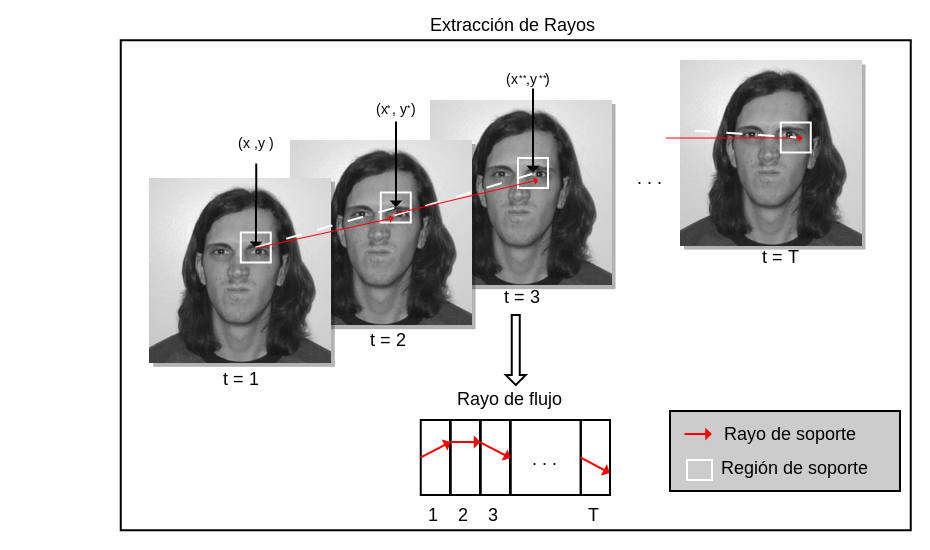
\includegraphics[width=10cm]{imagenes/Extraccion_de_rayos.png}
          		\caption{Representación de la extracción de rayos de un vídeo.}
            \end{figure}
        \end{frame}

        \begin{frame}{Extracción de micro-descriptores}{Normalización de rayos}
            \begin{figure}[bt]
        		\centering
                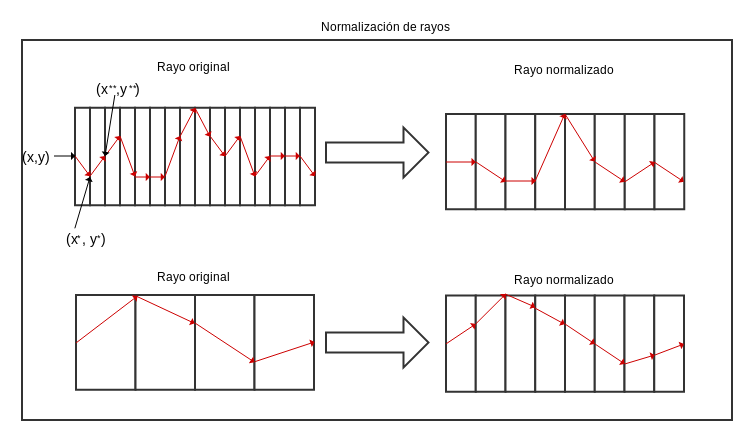
\includegraphics[width=10cm]{imagenes/normalizacion_de_rayos.png}
          		\caption{Normalización de rayos.}
            \end{figure}
        \end{frame}
    
    \subsection{Creación de macro-descriptores}
		\begin{frame}{Creación de macro-descriptores}{Vista general}
            \begin{figure}[bt]
        		\centering
                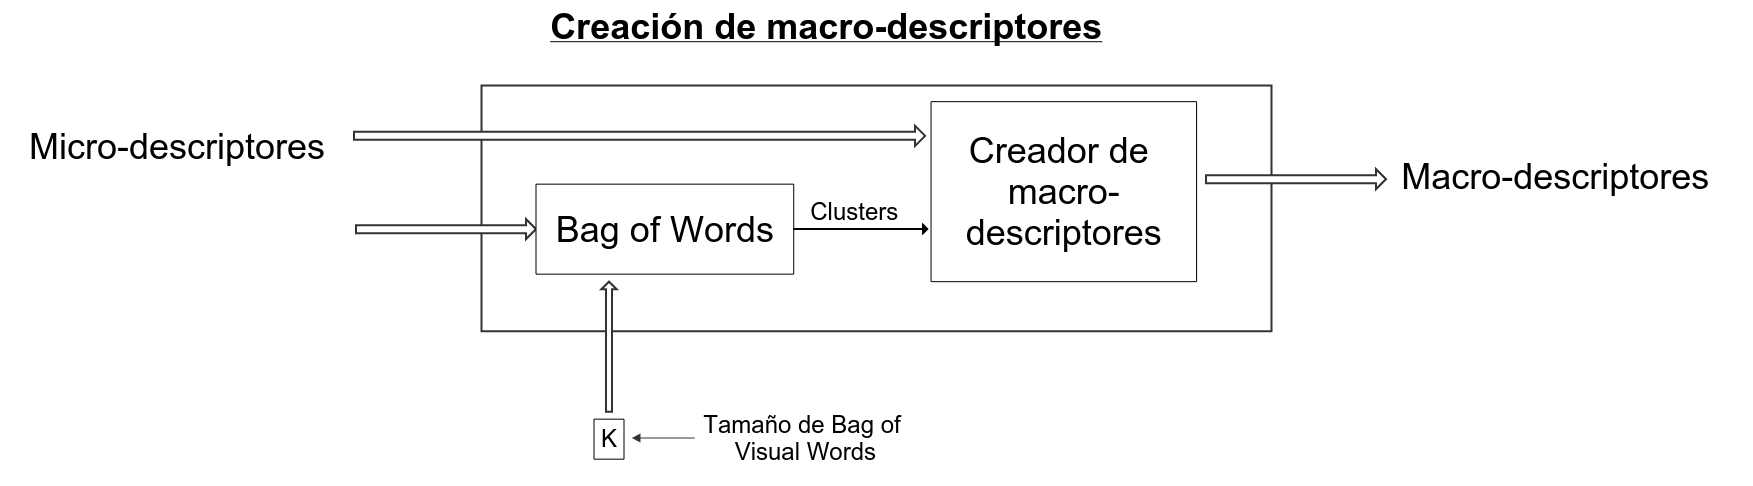
\includegraphics[width=7cm]{imagenes/Extractor_macrodescriptores_entrenamiento.png}
          		\caption{Creación de macro-descriptores entrenamiento.}
            \end{figure}
            
            \begin{figure}[bt]
        		\centering
                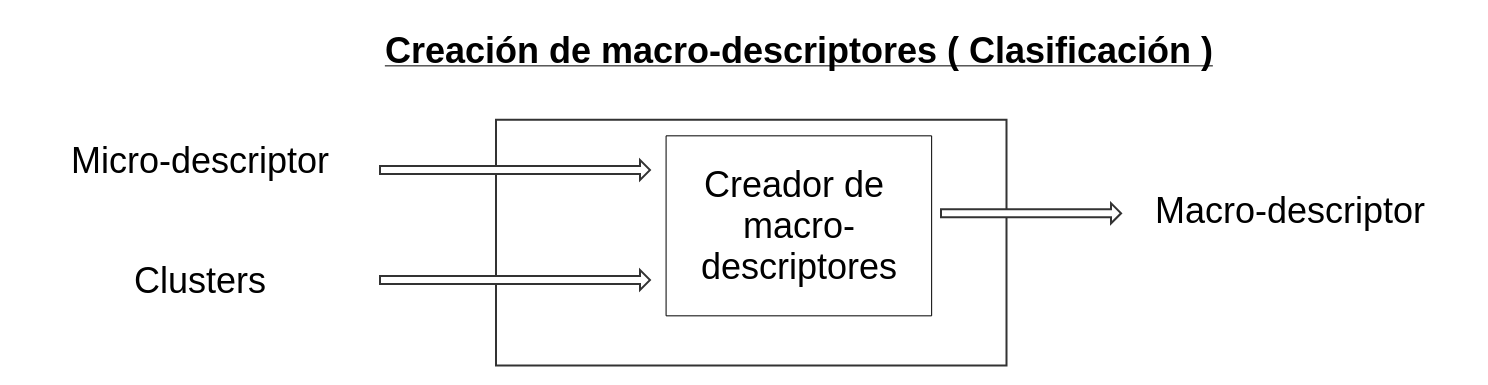
\includegraphics[width=7cm]{imagenes/Extractor_macrodescriptores_clasificacion.png}
          		\caption{Creación de macro-descriptores clasificador.}
            \end{figure}
        \end{frame}
        
        
        \begin{frame}{Creación de macro-descriptores}{Bag of Visual Words}
            \begin{equation}
  				\label{algoritmo:eq:dist}
				k^* = \arg \min_k \{\mathit{dist}(R(x,y),C_k)\},
			\end{equation}
            \begin{figure}[bt]
        		\centering
                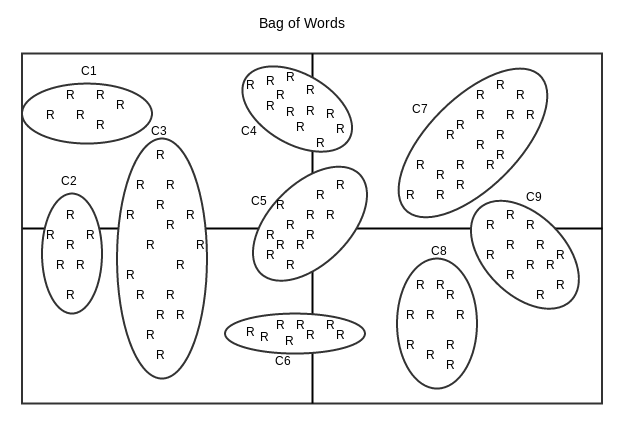
\includegraphics[width=7cm]{imagenes/bow_solo.png}
          		\caption{Representación gráfica del Bag of Visual Words.}
            \end{figure}
        \end{frame}
        
        \begin{frame}{Creación de macro-descriptores}{Creación del descriptor}
			\begin{equation}
				D_i(k) = \sum_{(x,y)\in\text{ROI}_i} \delta (R(x,y),k) \quad \forall k
			\end{equation}
			\begin{equation}
				 \delta (R(x,y),k) =  \begin{cases}
				 1 & \mbox{si }R(x,y)~\in~C_k\\
     			0 & \text{otro caso}
     			\end{cases}
			\end{equation}
		
			\begin{equation}
				\mathbb{D} = \cat_{i = 1}^{I} D_i, \quad \forall i
			\end{equation}				
		
		    \begin{figure}[tb]
        		\centering
                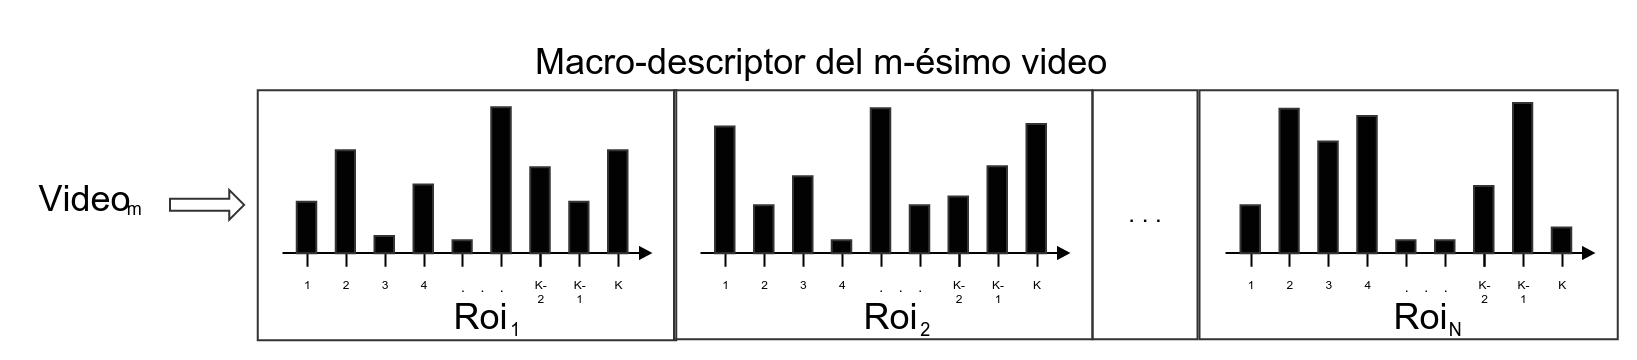
\includegraphics[width=7cm]{imagenes/macro-descriptor.png}
          		\caption{Construcción del macro-descriptor.}
            \end{figure}
        \end{frame}
    \subsection{Entrenamiento y clasificación}
    
		\begin{frame}{Entrenamiento y clasificación}{Vista general}
			  \begin{columns}[onlytextwidth]
   	 			\begin{column}{0.5\textwidth}
		            \begin{figure}[bt]
    			    			\centering
            		    		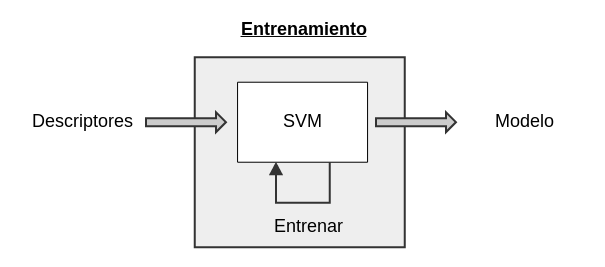
\includegraphics[width=6cm]{imagenes/Entrenamiento.png}
          				\caption{Diagrama de entrenamiento.}
            			\end{figure}
 				\end{column}
    				\begin{column}{0.5\textwidth}
		            \begin{figure}[bt]
        					\centering
        		        		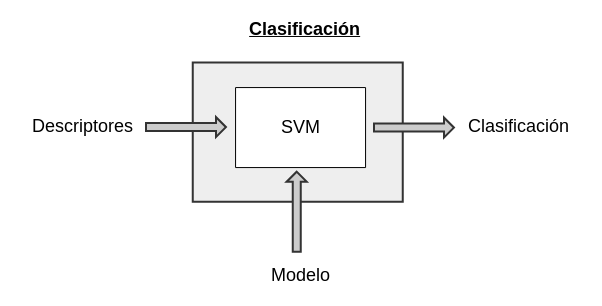
\includegraphics[width=6cm]{imagenes/Clasificacion.png}
        	  				\caption{Diagrama de clasificación.}
		            \end{figure}
        			\end{column}
 			  \end{columns}
        \end{frame}


		\begin{frame}{Entrenamiento y clasificación}{Support Vector Machines}
            \begin{figure}[bt]
        		\centering
                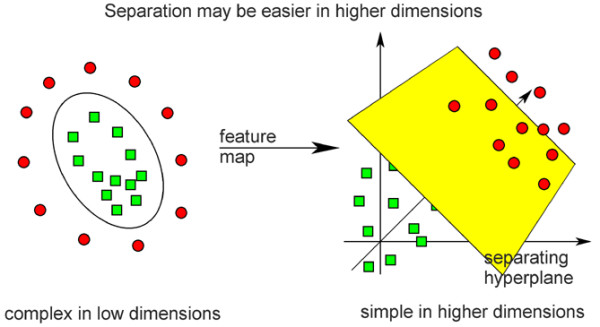
\includegraphics[width=8cm]{imagenes/svm.jpg}
          		\caption{Utilización de Kernel para el cambio de espacio.}
            \end{figure}
        \end{frame}
        
        \begin{frame}{Entrenamiento y clasificación}{Support Vector Machines}
            \begin{figure}[bt]
        		\centering
                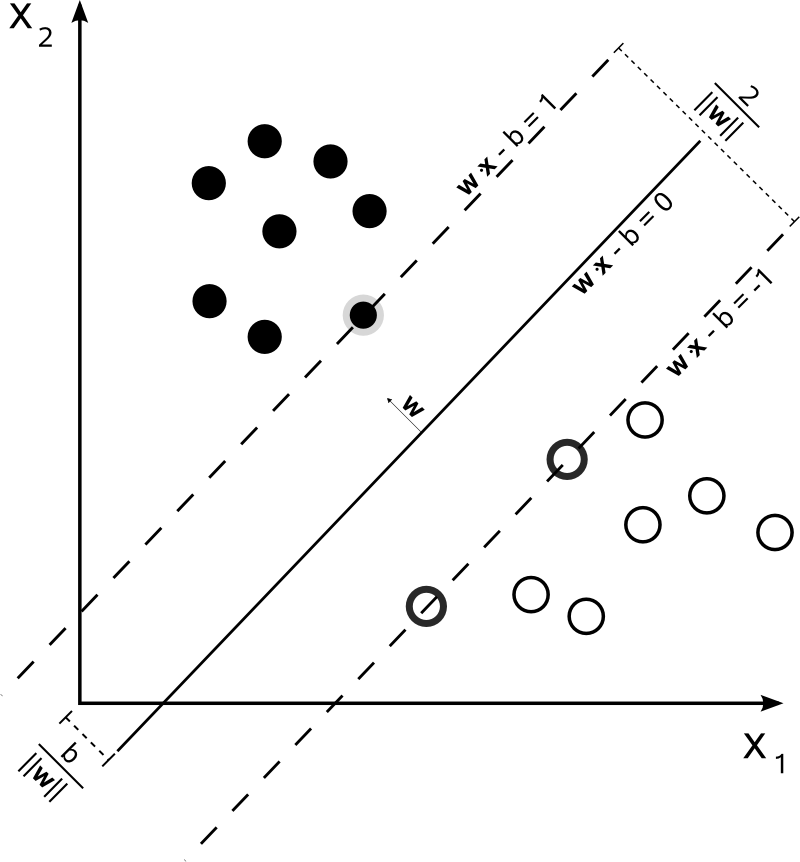
\includegraphics[width=5cm]{imagenes/support_vector_machines.png}
          		\caption{Support Vector Machines.}
            \end{figure}
        \end{frame}
        
        \begin{frame}{Entrenamiento y clasificación}{k-fold cross validation}
            \begin{figure}[bt]
        		\centering
                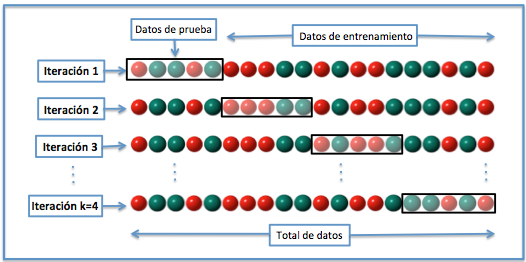
\includegraphics[width=7cm]{imagenes/K-fold.jpg}
          		\caption{k-fold cross validation.}
            \end{figure}
            \begin{equation}
            		Precision = \frac{|Videos~bien~clasificados|}{|Total~de~videos|} 
            \end{equation}
   
        \end{frame}
        
			        
        

\section{Trabajos futuros}
        \begin{frame}{Trabajos futuros}{Experimentos}
			\begin{enumerate}
				\item Codificación
					\begin{enumerate}
						\item Sin codificación
						\item Codificación LBP
						\item Codificación LDN
					\end{enumerate}
				\item Variables
					\begin{enumerate}
						\item Tamaño región de soporte $L$
						\item Variable de normalización $N$
						\item Cantidad de \textit{Clusters}
					\end{enumerate}
				\item Métricas de distancia.
			\end{enumerate}					        
        \end{frame}
    



% All of the following is optional and typically not needed. 
\section*{Preguntas}
	\begin{frame}{Gracias por su atención}
		\begin{center}
			¿Preguntas?
		\end{center}
	\end{frame}
	

\end{document}


